% !TeX root = ../main.tex
% Add the above to each chapter to make compiling the PDF easier in some editors.

\chapter{Introduction}\label{chapter:introduction}


With the clean energy transition currently taking place in Europe with ambitious targets for 2030 and beyond \cite{EU_RE_Targets_2023}, wind energy is playing a central role in that transition, with wind energy expected to rise to 50 \% in the EU energy mix. \cite{ConsiliumEU_Harnessing_Wind_Power_2024}
With wind energy thus expected to become the main contributer to the EU's energy production and large potentials identified for both onshore and offshore parks \cite{EEA_Wind_Energy_Potential_2009} attempts to optimize all parameters of windparks with even minor power efficeny improvement can be expected to yield significant returns in absolute power due to the scale of future wind energy production. 

Within the total generated power by wind energy lies the subproblem of optimizing the layout of wind farms. Here, the main goal is to reduce the negative impact that wake effects between wind turbines have on overall power generation, with yield reduction of up to $15\%$  mainly due to reduced wind speeds in wake regions. Optimizing the farm for overall minimal wake exposure between wind turbines can thus potentially significantly increase power yield. \cite{hou_review_2019} \cite{KIM2024123383} 

In practice, the problem reduces to placing wind turbines within a predefined zone, subject to the wind conditions as shown in \ref{fig:intro_plot}. These wind conditions can be assumed to be deterministic or (more accurately) as random variables, by considering probability distributions for variables like wind direction and wind speed.


\begin{figure}[h] 
	\centering
	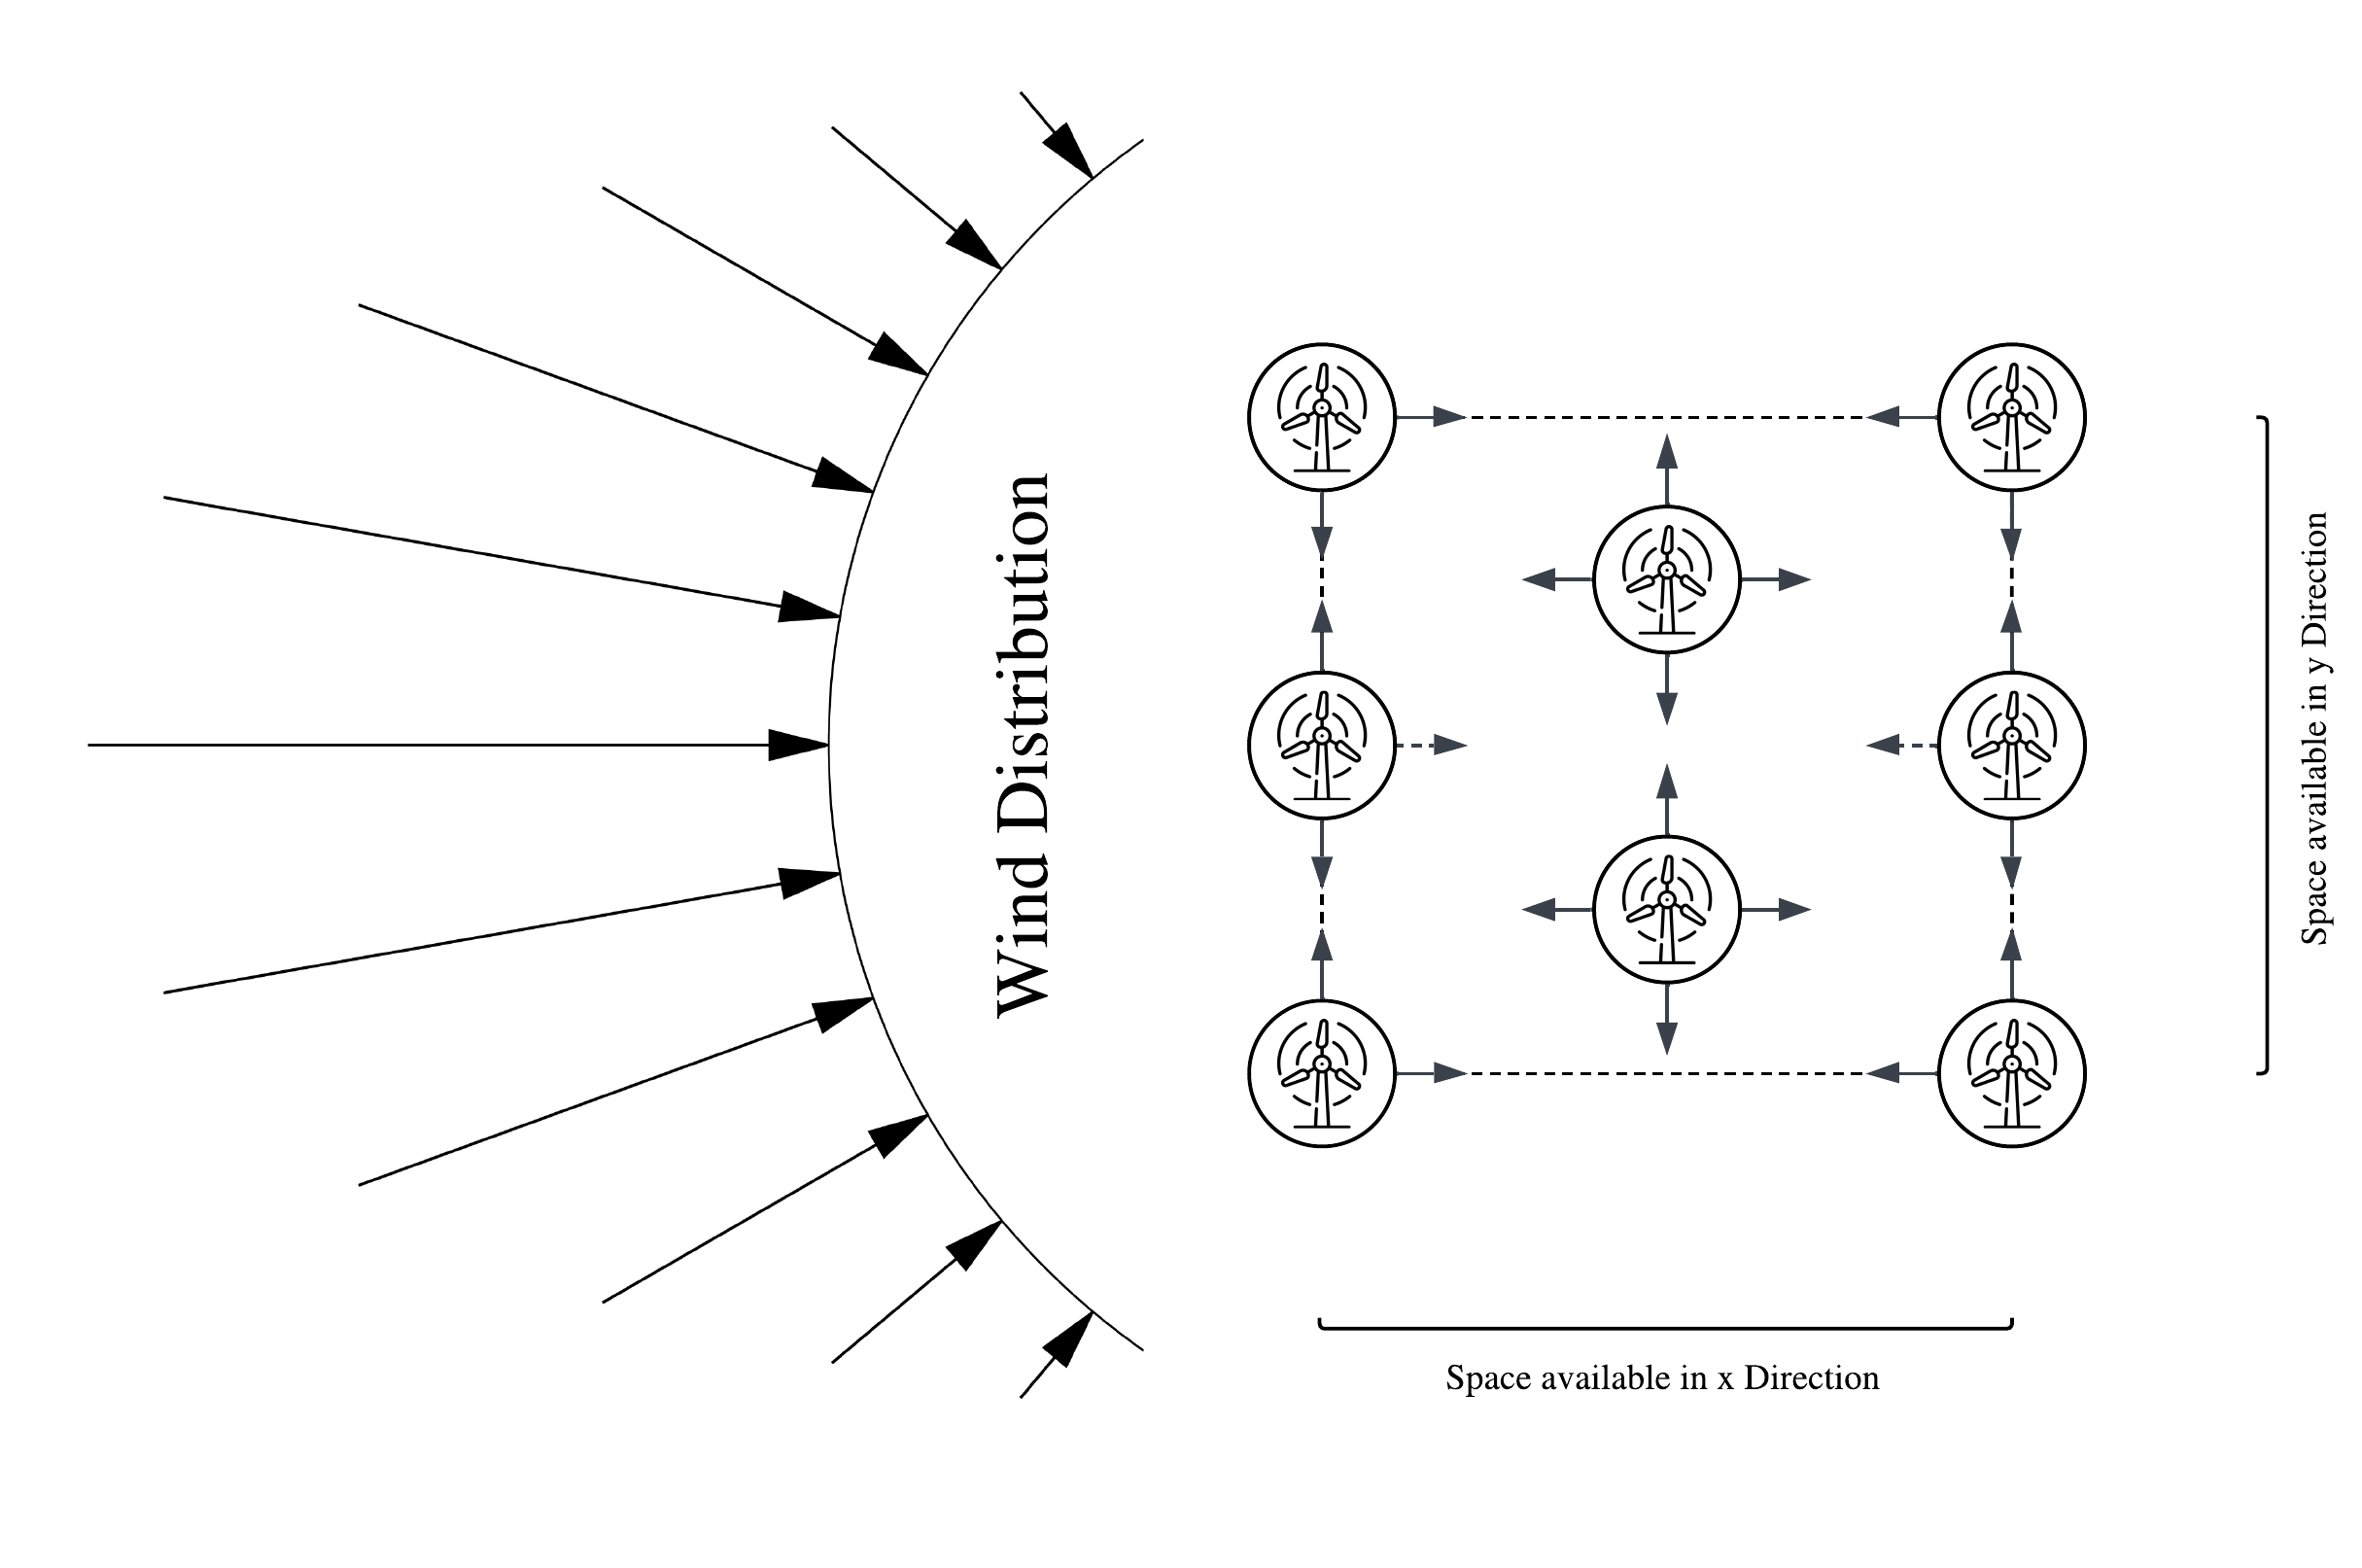
\includegraphics[width=1\textwidth]{figures/introduction/intro_plot.png} 
	\caption{Optimizing the total power output of a farm reduces to placing wind turbines within a set space for the farm, subject to the wind conditions at the given location}
	\label{fig:intro_plot}
\end{figure}

In mathematical terms, this problem can be expressed as the attempt to maximize the sum of power output across all turbines, e.g., maximizing total farm output, subject to the limitations of the defined space, which is assumed to be rectangular: 

\begin{align}
	\max_{\mathbf{x}, \mathbf{y}} & f_{Power}(x_i, y_i, wind_conditions) \\
	\text{s.t.} \quad 
	&  0 \leq x_i \leq X_{\max} \\
	&  0 \leq y_i \leq Y_{\max} \\
\end{align}

where:
\begin{itemize}
	\item \( (\Delta x, \Delta y) \) are the relative distances of the two turbines
	\item \( f_{Power, \text{NN}}(\Delta x, \Delta y)\) is a neural network (deterministic) approximating the total power output
	\item \(  X_{\max}, Y_{\max} \) define the maximal distance the two turbines can be placed apart
	\item \( d_{\min} \) is the minimum distance between the two turbines
\end{itemize}


This thesis is dedicated to a new approach for optimizing the placement of such fixed number of wind turbines in a predefined space, beginning with the two-turbine problem, e.g. the problem of optimally placing two turbines relative to each other. To solve this optimization problem, an extension to the Pyomo Python library is used, which allows the introduction of Neural Networks to the optimization problem as constraints. \cite{ALCANTARA2023120895} This extension allows for introducing a Neural Network to model the effects of wind turbine placement relative to each other on power production for the respective wind turbines. Introducing this model to the optimization problem defined in Pyomo then allows for the optimization of overall power production across all wind turbines in the wind park. The optimization problem in its simplest form can be defined as


To create a model optimally fit to the needs of the optimization problem, the model is trained on data specifically generated with the \href{https://www.nrel.gov/wind/floris.html}{FLORIS} wind farm simulation tool  for optimal coverage of the parameter space of the optimization. To simplify the problem, the surface below the turbines is assumed to be perfectly flat and an equal wind speed is assumed along the entire height of the turbines. Solving the problem can be seperated into two main Steps 

\begin{enumerate}
	\item \textit{Farm Power Model:} Generation of simulation data covering the parameter space and training a Neural Network model with power generation as output
	\item \textit{Optimization:} Setting up optimization problem, embedding of power model and solving
\end{enumerate}

This thesis is structured according to these two main steps, with a brief review of the state-of-the-art beforehand. 







